\documentclass{article}
\usepackage{graphicx}
\graphicspath{{images/}}
\usepackage{hyperref}
\title{TP 4A - Génie Logiciel
Programme Java intégrant modélisation UML, versionning (git)
et tests unitaires (Junit)
}
\author{Mathis Vaugeois - Tanguy Moriceau - Faustine Guillou}
\date{January 2023}

\begin{document}

\maketitle
\tableofcontents

\newpage
\section{Introduction}
\subsection{Context}

\subsection{Git}

Pour travailler en groupe, Nous avons décidé d'appliquer ce que nous avions appris en cours : Git. Nous avons mis proprement à jour nos comptes GitHub. Mathis a créé

\newpage
\section{Cahier des charges}
\subsection{Exercice 1}

\begin{figure}
    \centering
    \includegraphics[width=0.75\textwidth]{diagrammeClasse}
    \caption{Diagramme de Classe}
    \label{fig:mesh1}
\end{figure}

%\begin{figure}
    %\centering
   % \includegraphics[width=0.75\textwidth]{diagrammeSeq}
    %\caption{Diagramme de Séquence.}
    %\label{fig:mesh2}
%\end{figure}

%\begin{figure}
    %\centering
   % \includegraphics[width=0.75\textwidth]{diagrammeObj}
    %\caption{Diagramme d'Objet.}
    %\label{fig:mesh3}
%\end{figure}

1.
Voici notre diagramme UML \ref{fig:mesh1} que vous pouvez voir sur la page \pageref{fig:mesh1}.
\newline
2. Voici notre diagramme de séquence % \ref{fig:mesh2}
 que vous pouvez voir sur la page% \pageref{fig:mesh2}.
\newline
3. Nous pourrions aussi proposer un diagramme d'objet. Nous avons décidé le réaliser, le voici:
% \ref{fig:mesh3}
.Vous pouvez aussi le voir sur la page% \pageref{fig:mesh3}.


\newpage
\section{Code de départ}
\newpage
\section{Développement}
\subsection{Exercice 4 - Fusion}

\subsection{Exercice 5 - Tests}
\newpage
\section*{Référence}




\url{https://github.com/mathisvaugeois/TPBank-GenieLogiciel}

\end{document}